\subsection{App principale}
% Il punto di entrata del programma è l'activity \texttt{MainActivity} che contiene la mappa e i comandi per effettuare le misurazioni.

\subsubsection{ViewModel dei \textit{sampler}} \label{sec:MeasureViewModel}
Per ciascun \textit{sampler} è stato definito un ViewModel dedicato contenente le operazioni e le informazioni per ciascun tipo di misurazione.
In particolare, è stata definita una gerarchia di ViewModel come rappresentato in \cref{fig:viewmodel_hierarchy}.

\begin{figure}[H]
  \centering
  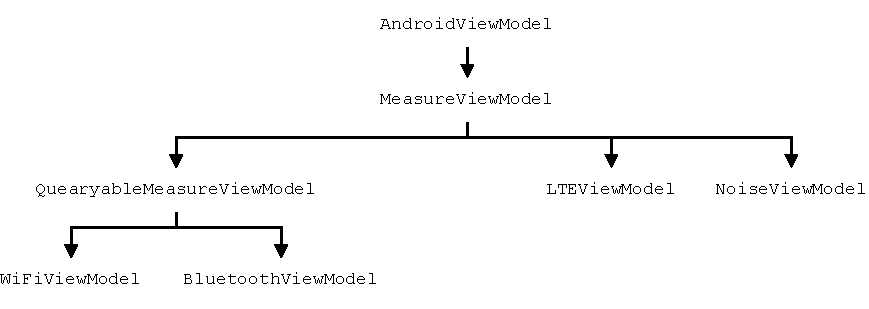
\includegraphics[width=\textwidth]{./img/viewmodel.pdf}
  \caption{Gerarchia dei ViewModel} \label{fig:viewmodel_hierarchy}
\end{figure}

La gerarchia ha come radice \texttt{AndroidViewModel} in quanto fornisce il \texttt{Context} dell'applicazione necessario per i \textit{sampler}.

La classe astratta \texttt{MeasureViewModel} fornisce tutte le informazioni utili per una tipologia di misurazione. Specificamente, contiene l'istanza del \texttt{WaveSampler} e i parametri quali: il range di qualità, il numero di intervalli, il numero di misure passate da considerare e un flag per indicare se caricare anche le misure condivise.
Vengono inoltre esposti i metodi per effettuare una nuova misurazione, ottenere la media delle misurazioni di una casella e caricare le impostazioni specifiche per il tipo di misura.
Da \texttt{MeasureViewModel} sono implementati \texttt{LTEViewModel} e \texttt{NoiseViewModel}.

\texttt{MeasureViewModel} viene poi estesa in un'ulteriore classe astratta \texttt{QuearyableMeasureViewModel} per rappresentare un tipo di misura a cui è possibile sottoporre un filtro di ricerca. È infatti richiesta l'implementazione di un metodo per elencare le possibili opzioni di ricerca e per cambiare la ricerca. Da questo tipo di ViewModel sono implementati \texttt{WiFiViewModel} e \texttt{BluetoothViewModel}, in entrambi i casi la ricerca si basa sul BSSID.


\subsubsection{MainViewModel}
Il ViewModel \texttt{MainViewModel} implementa la logica principale dell'applicazione. Contiene un'istanza di tutti i ViewModel dei \textit{sampler} (in un vettore) e ad ogni istante ne considera uno come attivo (identificato dall'indice del vettore). Inoltre, per ogni \textit{sampler} tiene traccia dello stato (in misurazione e non) e garantisce mutua esclusione per ogni singolo ViewModel in modo tale da evitare di avviare più misurazioni della stessa tipologia.

Attraverso dei \texttt{LiveData}, \texttt{MainViewModel} comunica alla view eventi come: l'inizio e la fine di una misurazione, la necessità di aggiornare la mappa ed eventuali situazioni di errore.

Inoltre, \texttt{MainViewModel} gestisce le scansioni periodiche (se attivate nelle impostazioni) utilizzando un \texttt{Handler} e il metodo \texttt{postDelayed}.

Bisogna infine notare che tutte le operazioni asincrone sono legate allo scope \texttt{viewModelScope} in modo tale che, in caso la view venisse ricreata, le operazioni in corso non vengono interrotte.


\subsubsection{MainActivity}
La \texttt{MainActivity} è il punto di entrata dell'applicazione e comprende la mappa e i comandi dell'utente.
Oltre a istanziare e interfacciarsi al \texttt{MainViewModel}, gestisce la richiesta dei permessi (richiedendo sempre un sottoinsieme minimale) e gli eventi riguardanti i cambiamenti di casella provenienti da \texttt{WaveHeatMapFragment}.

Inoltre, si occupa di avviare e fermare i servizi in background durante la fase di creazione e distruzione del proprio ciclo di vita.